\documentclass{standalone}
\usepackage[T1]{fontenc}
\usepackage[latin2]{inputenc}
\usepackage[english]{babel}
\usepackage{tikz}
\usepackage{times}
\usetikzlibrary{calc,through,backgrounds,positioning,fit}
\usetikzlibrary{shapes,arrows,shadows,calendar}
\begin{document}
 
\centering

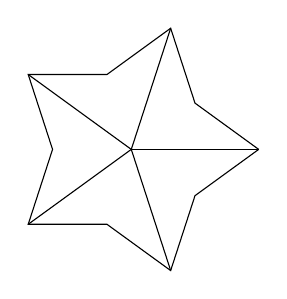
\begin{tikzpicture}[scale=1,inner sep=0.4mm]
\draw (0,0) -- (0:1.618) coordinate (p1);
\draw (0,0)  (36:1) coordinate (p2);
\draw (0,0) -- (72:1.618) coordinate (p3);
\draw (0,0)  (108:1) coordinate (p4);
\draw (0,0) -- (144:1.618) coordinate (p5);
\draw (0,0)  (180:1) coordinate (p6);
\draw (0,0) -- (216:1.618) coordinate (p7);
\draw (0,0)  (252:1) coordinate (p8);
\draw (0,0) -- (288:1.618) coordinate (p9);
\draw (0,0)  (324:1) coordinate (p10);
\draw (p1) -- (p2) -- (p3) -- (p4) -- (p5) -- (p6) -- (p7) -- (p8) -- (p9) -- (p10) -- (p1);
\end{tikzpicture}
\end{document}